\chapter{Experiments and Analysis}

In this chapter, we will present experiments to show the efficacy of the context discovery approach. Experiments are performed on real-world data from real users using a variety of social and personal media applications, public data sources. The motivation behind these experiments is to tag faces in thousands of personal photos taken by various people at different kinds of events. We will also perform experiments on generated data to simulate large scale use cases. Here, the motivation is to analyze the performance characteristics of the merge algorithm.

\section{Experiments on Real-World Data}
In this section, we analyze how CueNet helps tags personal photos taken at different events. For a given users, we will construct a dataset consisting of photos taken at a particular event. For each of these users, we will create a candidate set by aggregating people over personal, public and social data sources. In order to evaluate CueNet, we will attempt to reduce this candidate set, and analyze how many of the faces can be correctly tagged by this reduced set. We will also compare this performance over metrics like location based ranking, where candidates are ranked according to their last known location, and (if time permits) tie strength. Our final conclusion is that, in order to rank candidates for tagging faces in photos, CueNet provides an event-agnostic platform, where as other techniques perform inconsistently across different types of events.

\subsection{Setup}
We use photos taken during three different \textbf{types of events}: Social Parties, Academic Conferences and Trips. This diversity allows for different distributions of face tags across different aspects of a user's life. Social Parties generally tend to have close friends who are spatially co-located. Conferences tend to have people from different parts of the world, but those who are affiliated with the area of the conferences. Trips, cannot always rely on location as a useful metric and can involve people from either social, personal or professional circles from a user's life. 

For each event type, we collect multiple datasets from 6 different people. A \textbf{dataset} consists of multiple photos during the event, the user's personal information, which contains information from sources like Google Calendar, personal email and profile information from social networks like Facebook and Twitter. We also collect a person's social networking information which consists of tweets written by the user or their friend during the time the event was occurring, the social network itself (friends on Facebook and Twitter, along with their profile information). Conference proceedings are downloaded from DBLP and the conference website. Facebook events are also obtained and stored in our database. Besides, location databases like Yahoo Placefinder were used to geocode addresses and reverse geocode EXIF GPS coordinates. We assume that all photos have a valid EXIF tag, especially the timestamp and GPS coordinates. This assumption is not a very hard one, as almost all photos captured in the last two years are through iPhone or Android smartphones, which add reasonably accurate GPS tags and accurate timestamps (where the phone clock is synced with the cell tower). The domination of iPhone in the photo market is shown in figure \ref{fig:flickr-camera-popularity}. The ground truth was annotated by the user with our annotation interface. For each photo, an annotation consisted of the ID of the person in the candidate set in it. Face verification was achieved initially with Face.com, but after their service was discontinued, we used the web service, Automatic Face Systems, maintained by Neeraj Kumar. After this service was terminated, we resorted to manual face verification. We use the manual verification for the experiments described below, unless otherwise mentioned.

\begin{figure}[t]
\centering
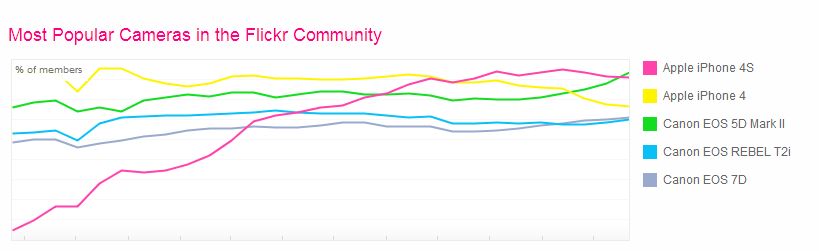
\includegraphics[width=0.9\textwidth]{media/flickr-camera-popularity.png}
\caption{Popularity of iPhone at Flickr.com (October 2011).}
\label{fig:flickr-camera-popularity}
\end{figure}

In order to construct a \textbf{candidate set} for each dataset, we construct a so-called \texttt{CandidateSet}. A \texttt{CandidateSet} data structure performs two functions. It is a persistent set of candidates each of which have a unique identifier. Second, each data source, which has its own identifier for a candidate can look up the candidate set with this identifier to obtain the candidate set identifier. Here is an example of a simple candidate set:

\begin{verbatim}
[
{csid: 1010-poqs, name: `Arjun Satish', email: `arjun@uci.edu', 
                                        email: `arjun.satish@gmail.com',
                                        facebook-id: `656563332'}
{csid: 2010-pasd, name: `Ramesh Jain', email: `jain@ics.uci.ed',
                                       name: `Dad',
                                       email: `jain49@gmail.com',
                                       facebook-id: `10004290384'}
{csid: 1255-juen, name: `Peter Boncz', confid: `cf-12-candidate-322'}
{csid: 7585-kdye, name: `Amarnath Gupta', email: `gupta@sdsc.edu',
                                          twitter: `aguptasd'}
{csid: 1111-bmel, name: `Arjun', twitter: `@wicknicks'}
]
\end{verbatim}

The above snippet is a part of the candidate set created during the tagging of my personal photos. A \texttt{CandidateSet} is a multimap where the keys are the unique IDs (shown as csid above). The values are a list of key-value attribute pairs. The key could be a global key, such as name or email address, which can be added by any data source. In the above example, different sources could contribute different names for the same entity. Same values for the same key are not duplicated. The list could contain keys which are local to a data source, for example the Facebook identifier key: \texttt{facebook-id}. This primarily helps in querying the candidate set to obtain a reference to the candidate during the discovery phase. 

The construction of the \texttt{CandidateSet} happens when the system is brought up. For each user, a unique \texttt{CandidateSet} is created, or loaded if it exists on disk. In order to create it, each data source is probed individually to provide a list of unique persons. The data source mediator checks if the user already exists in the \texttt{CandidateSet} through its local primary jkey. If he does, it adds additional key value pairs to the attribute list. If a candidate corresponding to its primary key does not exist, a new candidate is created in the set, and the local primary key is added as an attribute pair. This technique will fail to merge different identities of people if they use multiple email addresses or do not store email information on social networks. Thus, we create a merge file, which lists a set of merges between candidates. In the above example, we will use this functionality to combine the entries with IDs \texttt{1111-bmel} and \texttt{1010-poqs} into a unified candidate. This guarantees that context discovered for one online identity is propagated to other identities of the same person.

We use 1889 photos taken at 17 different events in our face tagging experiment. Each photo contains one or more faces. We will denote each dataset as `Di' (where 1 $\leq$ $i$ $\leq$ 17 for each dataset). Table \ref{tbl:unique-persons} describes each dataset in terms of number of photos, unique annotations in ground truth, the year they were captured and the type of the event. 

\begin{table}[h]
\begin{center}
\begin{tabular}{ |c|p{1.5cm}|p{1.5cm}|c|p{2.5cm}|c| }
  \hline
  \texttt{Dataset} & \texttt{Unique People} & \texttt{No.\ of Photos} & \texttt{Year} & \texttt{CandidateSet Size} & \texttt{Event Type}\\
  \hline
     D1  &  43   &   78   &  2012  &  660   & conference \\
     D2  &  24   &   108  &  2012  &  660   & conference \\
     D3  &  6    &   16   &  2010  &  660   & conference \\
     D4  &  7    &   10   &  2010  &  660   & conference \\
     D5  &  36   &   80   &  2009  &  660   & conference \\
     D6  &  18   &   65   &  2013  &  660   & conference \\
     D7  &  7    &   11   &  2013  &  660   & conference \\
     D8  &  12   &   25   &  2009  &  1894  & conference \\
     D9  &  14   &   65   &  2011  &  215   & party \\
    D10  &  13   &   131  &  2010  &  561   & party \\
    D11  &  6    &   85   &  2008  &  656   & party \\
    D12  &  50   &   74   &  2012  &  1049  & party \\
    D13  &  19   &   330  &  2009  &  691   & party \\
    D14  &  14   &   363  &  2009  &  711   & trip \\
    D15  &  2    &   208  &  2010  &  715  & trip \\
    D16  &  4    &   217  &  2011  &  711  & trip \\
    D17  &  7    &   23   &  2011  &  584  & trip \\
  \hline
\end{tabular}
\caption{Profile of datasets used in the experiments.}
\label{tbl:unique-persons}
\end{center}
\end{table}

We divide the sources into different categories to facilitate a more general discussion. The categories are ``Personal Information" (same as Owner Information in section \ref{sec:discovery-algorithm}), ``Event sources", and ``Social Networks". Event sources include Facebook events, Yahoo Upcoming web service, our conference events database among other sources. Social networks include Facebook's social graph. Personal information contained information about the user, and a link to their personal calendars. An annotation is considered ``Out of Context Network" if it is not in any of these sources.

\begin{figure}[t]
\centering
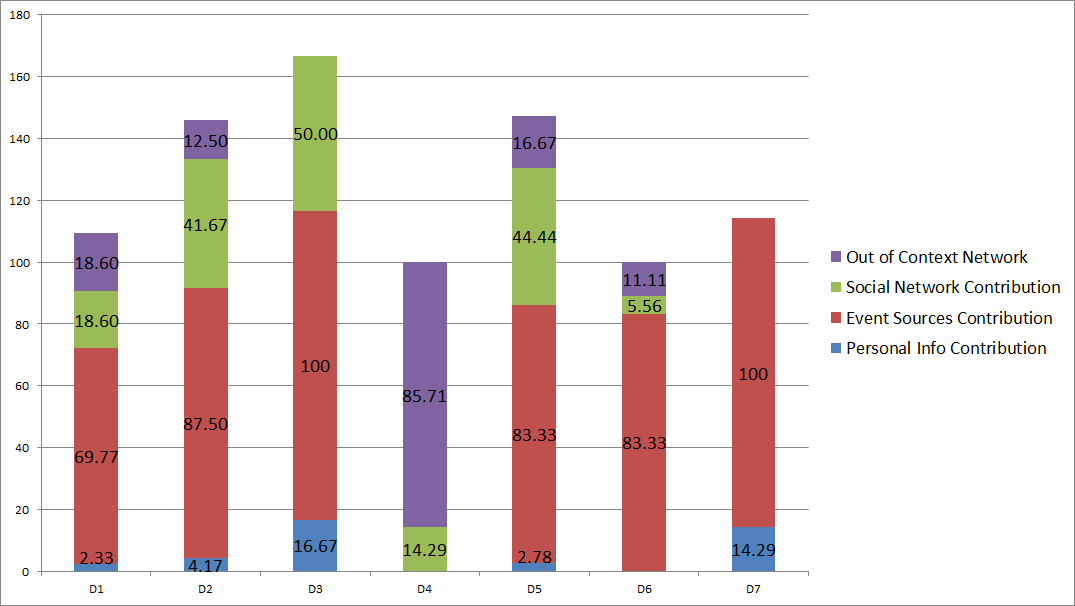
\includegraphics[width=0.9\textwidth]{media/gt-distro-stacked-2.png}
\caption{The distribution of annotations in the ground truth for conference photos across various sources.}
\label{fig:src-cand-distribution}
\end{figure}

Figure \ref{fig:src-cand-distribution} shows the distribution of the ground truth annotations of the conference datasets across various sources, for each dataset. For example, the bar corresponding to D2 says that 87.5\% of ground truth annotations were found in event sources, 41.67\% in social networks, 4.17\% in personal information and 12.5\% were not found in any source, and therefore marked as ``Out of Context Network". From this graph it is clear that event sources contain a large portion of ground truth annotations. Besides D4, a minimum of 70\% of our annotations are found in event sources for all datasets, and for some datasets (D3, D7) all annotations are found in event sources. The sum total of contributions will add up to values more than 100\% because they share some annotations among each other. For example, a friend on Facebook might show up at a conference to give the keynote talk.

\subsection{Individual List Sizes in a Dataset}
First, we look at how CueNet reduces the number of possible candidates for all photos in a dataset. For this setup, the complete candidate set $L$, contained 1894 labels (total number of people present at the conference, user's emails and social graph). The figure \ref{fig:exp-vldb-all-cx} shows various statistics for each photo, which includes the maximum size of the list which was generated by the discovery algorithm, the actual number of people in the photos, the number of true positives and false positives. As it can be seen, the size of the discovered set $S$, never exceeded 12. This is 0.5\% of the original candidate list. Because the total number of possible participants (list size) was low, our False Positive rate (FP) was very low too. Most of the false positives were due to profile orientation of faces or obstructions (this was because the face detector was smart enough to pick up profile faces, but verification worked better only on frontal faces).

\begin{figure}[t]
\centering
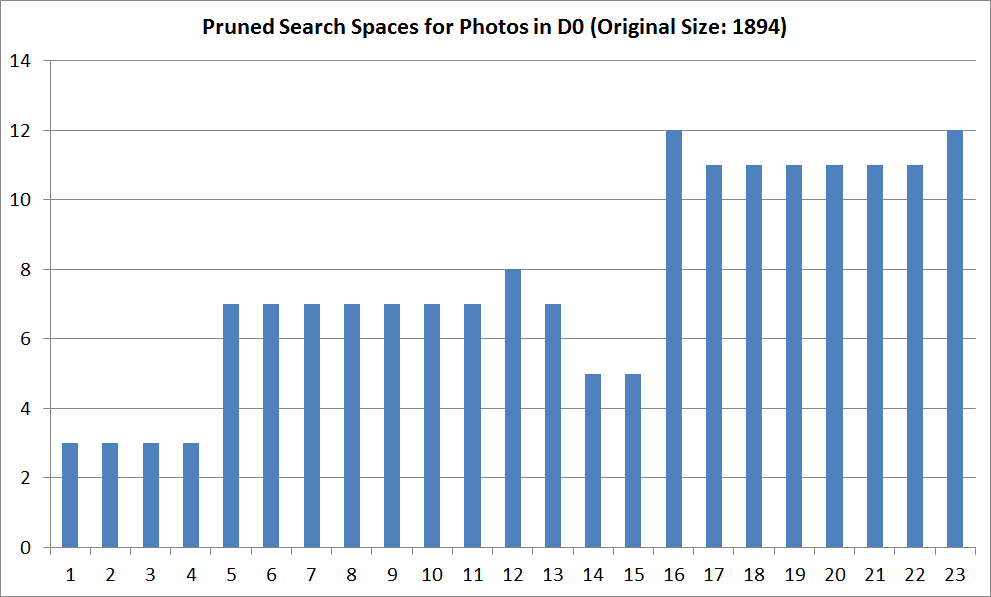
\includegraphics[width=0.9\textwidth]{media/reduced-list-sizes-d0.png}
\caption{Pruned search space for photos in conference dataset D8.}
\label{fig:exp-vldb-all-cx}
\end{figure}

\subsection{Results using Context Discovery}
In order to evaluate 17 different datasets, we perform the following modification on each dataset. For a dataset, we select the photo with all annotations, and attempt to tag it. The numbers seen below will reflect the results for such a photo. Alternatively, the numbers below can be interpreted as tagging the event itself, and not individual photos. We do this modification to reduce the number of graphs drawn per experiment. We define a \textbf{hit} as a correctly tagged face. Figure \ref{fig:exp-cx-hits} shows the hits for datasets using the context discovery algorithm. The blue bars show the number of unique faces in the dataset. As we can see the number of hits is equal to the number of unique faces, which implies that our context discovery algorithm was able to find the correct face tags for almost all datasets. Only for dataset 4, this difference is significant. This is because there was no contextual information related to the people in this dataset.

\begin{figure}[t]
\centering
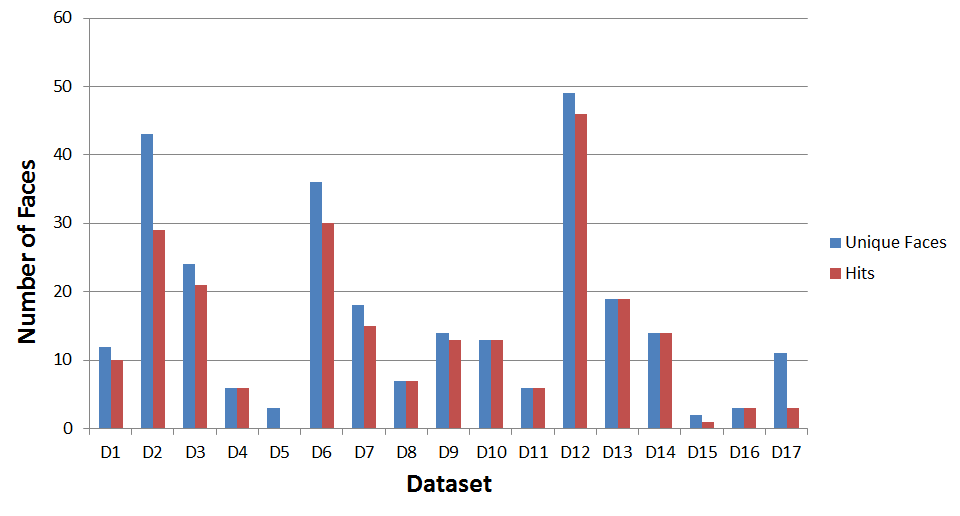
\includegraphics[width=\textwidth]{media/chapter5/axis/cx-unique-faces-hits-all-datasets.png}
\caption{Hit counts for all datasets using Context Discovery Algorithm.}
\label{fig:exp-cx-hits}
\end{figure}

Most of the datasets contain hundreds of candidates. If we have to perform face verification on all datasets, then the discovery algorithm is not performing effectively. The fewer the number of verifications, the better the pruning power of the algorithm. In order to quantify this, we introduce the metric \textit{Verification Ratio}, which is simply the number of verifications done per candidate in the \texttt{CandidateSet}. If this number is equal to 1, that means we have performed a very large number of verifications. The closer it is to 0, the fewer the number of verifications that were done. This ratio also enables us to compare the differences across dataset, where the number of candidates varies. As it can be seen in figure \ref{fig:exp-cx-verification-ratio}, the verification ratio never exceeds 19\% (the maximum value being 18.3\%).

\begin{figure}[t]
\centering
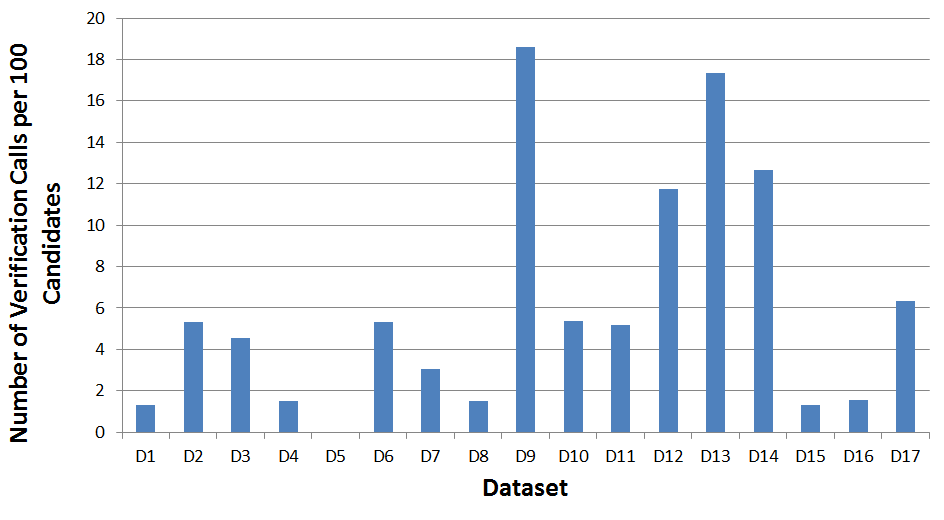
\includegraphics[width=\textwidth]{media/chapter5/axis/cx-verification-ratio-all-datasets.png}
\caption{Verification Ratio (x 100) obtained using the Context Discovery Algorithm.}
\label{fig:exp-cx-verification-ratio}
\end{figure}

In order to compare these results, we perform a tagging experiment using location information alone. Candidates are ordered according to their last known location, and presented to the user in the same style as the information presented with the context discovery algorithm. In this case, it must be noted that some users do not have location information related to them, and are excluded from the candidate set. The effect of this fact is seen in the reduced hit count seen using location information.

% \begin{figure}[ht]
% \begin{minipage}[b]{0.45\linewidth}
% \centering
% 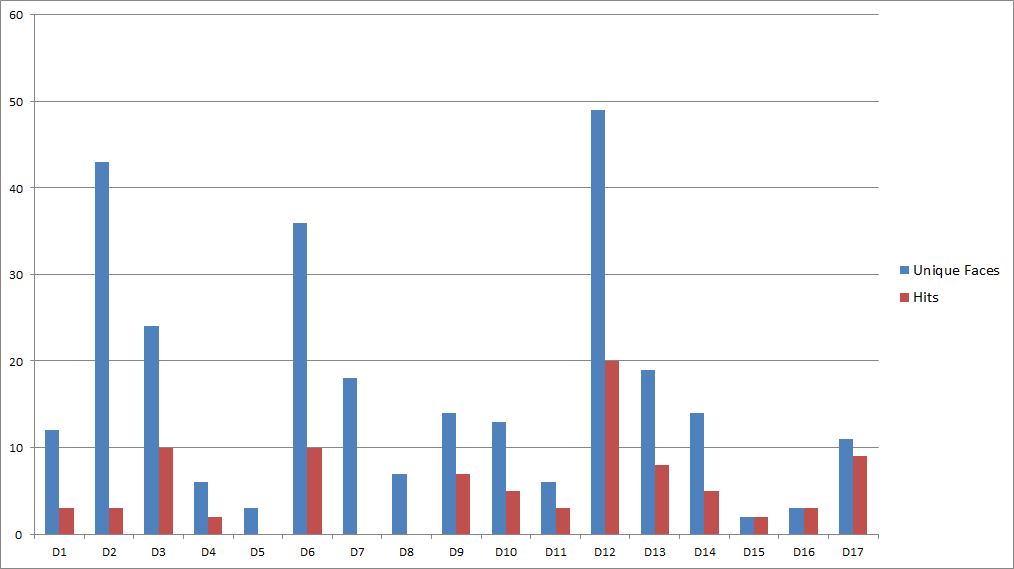
\includegraphics[width=0.9\textwidth]{media/chapter5/loc-unique-faces-hits-all-datasets.png}
% \caption{Hit counts for all datasets using Location only.}
% \label{fig:exp-loc-hits}
% \end{minipage}
% \hspace{0.5cm}
% \begin{minipage}[b]{0.45\linewidth}
% \centering
% 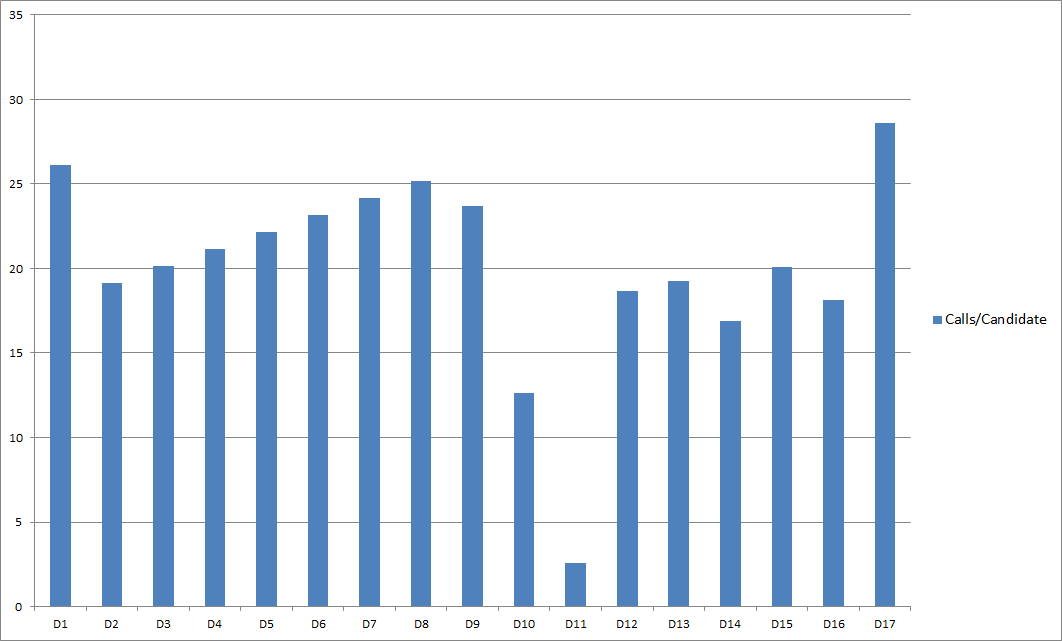
\includegraphics[width=0.9\textwidth]{media/chapter5/loc-verification-ratio-all-datasets.png}
% \caption{Verification Ratio (x 100) for all datasets obtained using Location only.}
% \label{fig:exp-loc-verification-ratio}
% \end{minipage}
% \end{figure}

\begin{figure}[ht]
\centering
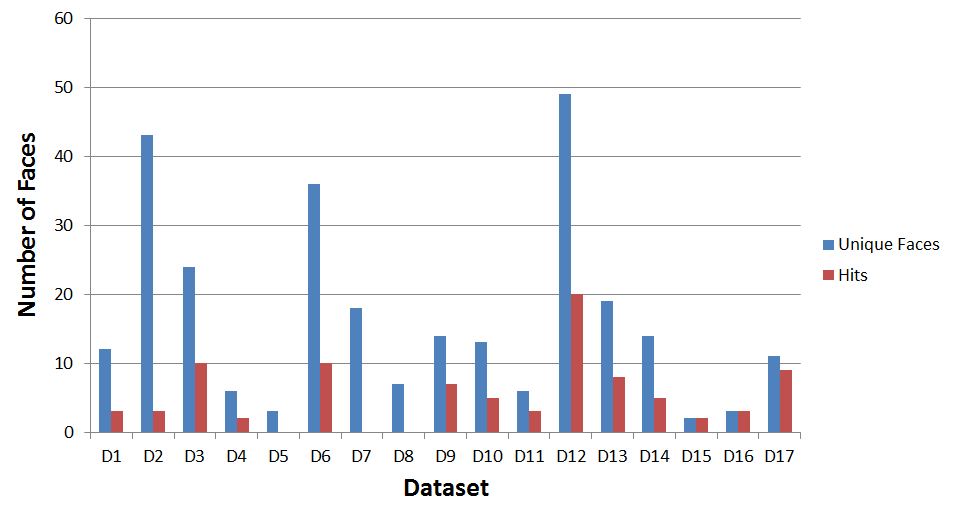
\includegraphics[width=\textwidth]{media/chapter5/axis/loc-unique-faces-hits-all-datasets.png}
\caption{Hit counts for all datasets using Location only.}
\label{fig:exp-loc-hits}
\end{figure}

Similarly, we measure the verification ratio using location only. The results in figure \ref{fig:exp-loc-verification-ratio} show that the maximum number has now increased to almost 29\%. 

\begin{figure}[h!]
\centering
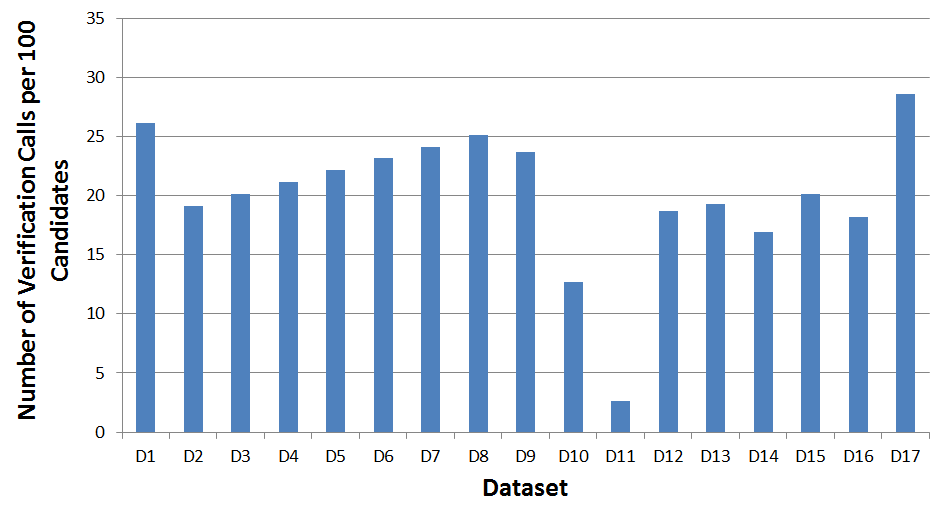
\includegraphics[width=\textwidth]{media/chapter5/axis/loc-verification-ratio-all-datasets.png}
\caption{Verification Ratio (x 100) for all datasets obtained using Location only.}
\label{fig:exp-loc-verification-ratio}
\end{figure}

% \begin{figure}[t]
% \centering
% 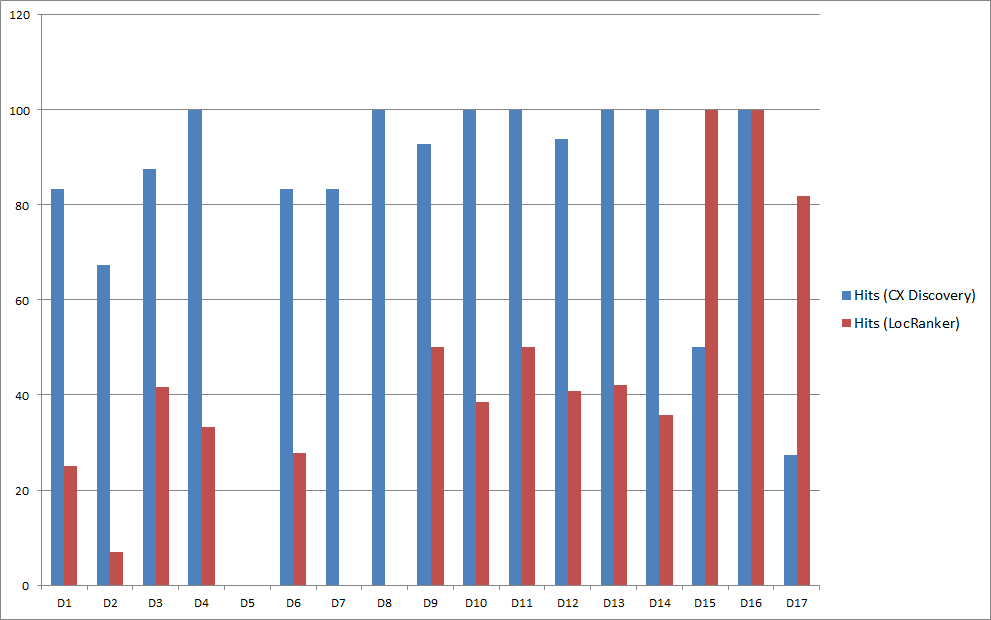
\includegraphics[width=0.9\textwidth]{media/chapter5/hits-ratio-comparison-all-datasets.png}
% \caption{Comparing Hits Ratio (x 100) for all datasets.}
% \label{fig:hits-ratio-comparison}
% \end{figure}

In figure \ref{fig:hits-ratio-comparison}, we compare the \textbf{hits ratio} of the context discovery algorithm with the location based algorithm. The hit ratio is the number of hits per unique face in a dataset. As it can be seen, the context discovery algorithm outperforms the simple location based ranking algorithm. The more important insight in this graph is that the context discovery algorithm performs \textbf{consistently across different types of events}, whereas the location based metric is good only for the party events. This was because in such social gatherings, participants lived closed to the location of the event. And therefore, ranked very highly when only location was used as context. Figure \ref{fig:verification-ratio-comparison} compares the different verification ratios. The relatively lower numbers for the context discovery algorithm indicate its superior ranking over the location based algorithm. Again, the important thing is to note its \textbf{performance across event types}. 

\begin{figure}[h!]

\begin{minipage}[b]{\linewidth}
\centering
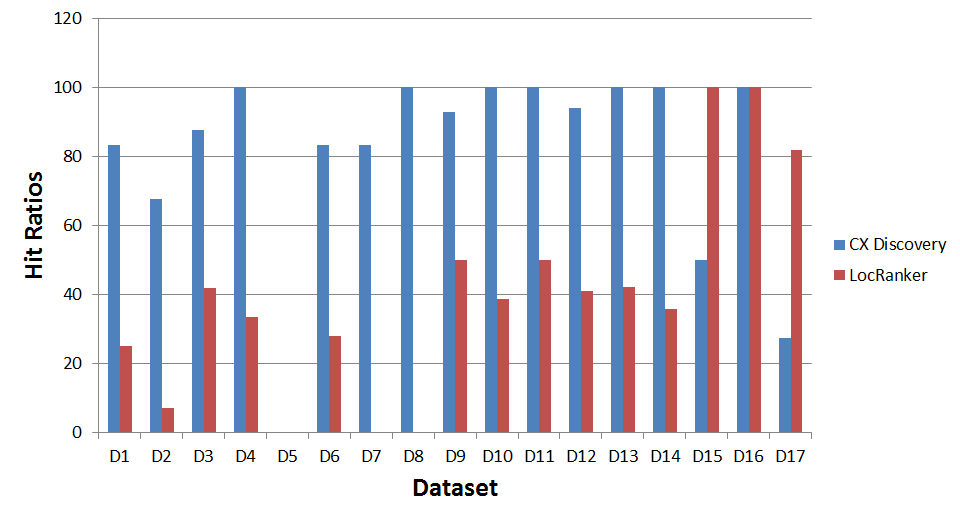
\includegraphics[width=\textwidth]{media/chapter5/axis/hits-ratio-comparison-all-datasets.png}
\end{minipage}
\caption{Comparing Hits Ratio (x 100) for all datasets.}
\label{fig:hits-ratio-comparison}

\vspace{0.5cm}

\begin{minipage}[b]{\linewidth}
\centering
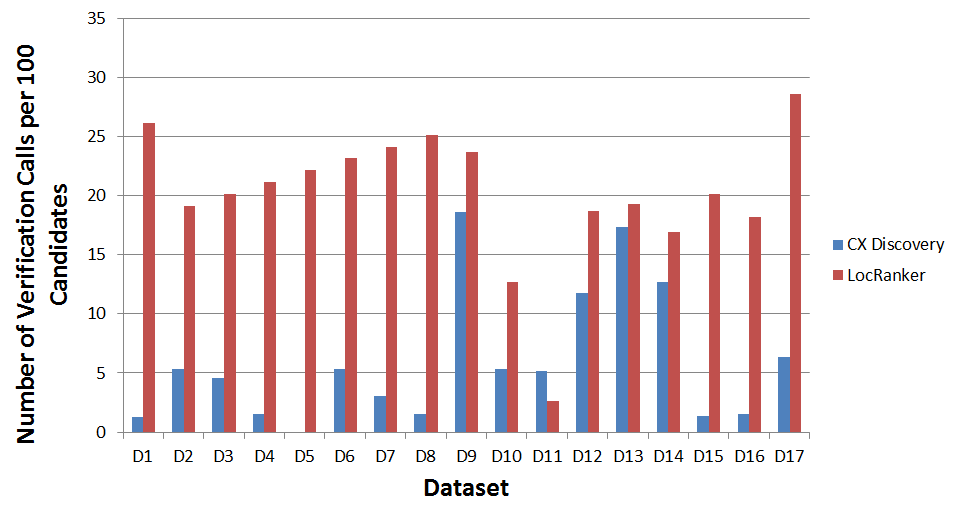
\includegraphics[width=\textwidth]{media/chapter5/axis/verification-ratio-comparison-all-datasets.png}
\end{minipage}
\caption{Comparing Verification Ratio (x 100) for all datasets.}
\label{fig:verification-ratio-comparison}

\end{figure}

\subsection{Conclusion}
We summarize the results of this experiment as follows. The context discovery algorithm performs consistently well across different types of events. Depending on the type of the event, it discovers the best data sources and ranks the candidate set in the appropriate way. For a single dataset, the ranking of candidates can significantly vary depending on who has been tagged in the photo. There are many research opportunities to propagate context across photos taken at different events and within the same event. We present such an context propagation algorithm in chapter 6.

\section{Importance of Individual Sources}

So far, we have used different sources, without evaluating their individual contributions to the discovery process. In order to empirically study, we will perform the tagging experiments without each one of the sources. And for each such run of the algorithm, tabulate the hit counts. This will give us an insight into the contribution of each source. Figure \ref{fig:source-benefits} plots the hit counts for two conference datasets(D2, D8), two party (D9, D12) and two trip (D14, D16) datasets from our original collection. The hit counts are normalized to 100, to allow for easy comparison. In the graph, the source `Facebook' collectively refers to event and social network information obtained from the website. The source `Conference' refers to the keynotes, sessions, lunch/coffee breaks and talk information obtained from conference proceedings. For each dataset, figure \ref{fig:source-benefits} plots the hit counts when one of the sources is absent.

\begin{figure}[t]
\centering
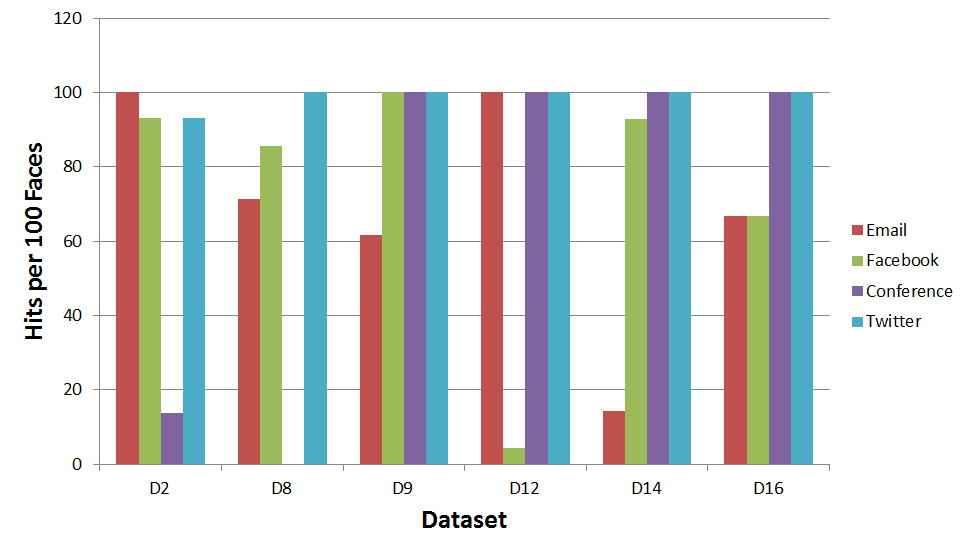
\includegraphics[width=\textwidth]{media/chapter5/axis/source-benefits.png}
\caption{Reduction in hit counts observed as a data source is removed.}
\label{fig:source-benefits}
\end{figure}

Figure \ref{fig:source-benefits} shows that the Twitter source is least important for most datasets. This could be because a variety of our users do not use the twitter service during their personal events. Personal events also do not have hashtags because of which it becomes hard for correlate which tweets correspond to events the user is participating. During the presence of such hashtags, their role becomes more prominent (in dataset D2), but not by a large amount. The conference source is most useful to tag photos taken at conferences. But shows no contributions otherwise. This is understandable as the source is curated exclusively for such events, and for none other. 

The role of Facebook and Email are the most interesting parts of this experiment. The Facebook social network and their events repository are extremely valuable in tagging photos. Almost all datasets lose a portion of their tags if this source is not considered. Although, it does not affect all datasets, but on average, worse damage is caused when photos are tagged without email sources. The average loss being 31.013\% for emails and 26.2184\% for Facebook. This difference was due to the fact that people almost always correspond with emails before or after an event. As we will see in the next section, there are certain reasons which make Email even more valuable than Facebook for our current application. It should be noted that we are computing the hit count at the end of all iterations. It might happen that a source provides valuable context in the first iteration, which leads to discovering many tags in the later iterations. Although this source itself provided very little context, its utility was very high.

\section{Time of Context Discovery}

In all our experiments, we did not mention the time of context discovery - at what point in time should we run context discovery algorithms to gather most context. Since sources are constantly evolving, there must be some time after the photo is taken, that is best to query source APIs or download them to local databases. The trivial answer is to take as long as possible after the photo is taken to access context. In this section, we will look at some specific instants where this is not true.

Consider dataset D2, which consisted of photos taken at a conference. During this conference, we queried Twitter's real time search API to gather tweets from people who were attending the conference. Twitter imposes a limit of searching content which was published up to two weeks ago. This restriction limits the use of the Twitter source for all events which had occurred in the past, or be limited to the followers of a user on the network. Thus, to obtain best response tweets must be obtained in real time or within two weeks, which can be very challenging if event hashtags are not known in advance.

Similarly, when we consider conferences photos in D8, tagging of photos immediately as they are captured, yields very low results. This is because almost all context was generated a few hours or days after the photos were captured. Discovering any sooner left us with all the conference attendees, out of which only very few were previous acquaintances of the owner. The severity of this problem is reduced due to the fact that email is very easily indexed by time, and all email protocols provide temporal predicates in their queries. Thus, updates to a owner's email source can be very easily routed to a discovery algorithm to update its status.

In our previous experiments, the Facebook sources have shown to be very useful. This is not true in the case of the social network. The Facebook API only provides the latest snapshot of the network. There is no way to query `the state of relationships at time, T'. The location based ranking step in our algorithm suffered due to this. People who were ranked highly because of their spatial proximity to an event a year ago are no longer ranked high because they have updated their location on Facebook (people moving away after changing jobs or graduating from school). Also people delete their accounts which may cause the hit count to reduce. Hence, although social information is very important, it cannot be used to tag photos taken long time ago, as the information on it is not relevant to the photo. On the other hand, event information on social network is still useful. From an engineering perspective, many companies such as CueUp download snapshots of Facebook networks on a nightly basis to circumvent such problems.

In short it is clear that the best time to tag photos is not immediately and a long while after it was captured. There exists a window which is the best time to gather context for a given photo and use it for tagging. In our work, we assume that the context sources do not change. For applications, where this is not true, discovery operations will be repeated as the content of the source change. 


% Now, lets look at reduction obtained in state space with the discovery algorithm. The total number of people in our experiment universe is 660. By statically linking the sources, we would expect the search space to contain 660 candidates for tagging any of the datasets. However, the context discovery algorithm reduced the size of the search space as shown in table \ref{tbl:search-spaces}. The search space varies from 7 people in D7 (1\%) to 338 people in D2 (51\%). We denote the term hit rate as the percentage of true positives in the search space. Even if our search space is small, it might contain no annotations from the ground truth, leading to poor classifier performance. The hit rates are also summarized in table \ref{tbl:search-spaces}. For D4, the algorithm found no event sources (as seen in figure \ref{fig:src-cand-distribution}), and therefore constructed a search space which was too small, thereby containing none of the ground truth. With the exception for D4, the hit rate is always above 83\%. We observe an overall reduction in the search space size, with a high hit rate for majority of the datasets. 

% \begin{table}[h]
% \begin{center}
% \begin{tabular}{ |c|p{2.5cm}|c| }
%   \hline
%   \texttt{Dataset} & \texttt{Reduced Search Space Size} & \texttt{Hit Rate}\\
%   \hline
% %  D0 & TBD & TBD \\
%   D1 & 42 & 83.72\%\\
%   D2 & 338 & 87.5\%\\
%   D3 & 231 & 100\%\\
%   D4 & 1 & 0\%\\
%   D5 & 254 & 83.33\%\\
%   D6 & 20 & 88.89\%\\
%   D7 & 7 & 100\%\\
%   \hline
% \end{tabular}
% \caption{Sizes of Search Space for each dataset.}
% \label{tbl:search-spaces}
% \end{center}
% \end{table}

% We now investigate the role of different context sources in the discovery algorithm. If an entity in the search space was merged into the event graph by an event source, they are said to be ``contributed" from it. We profiled our algorithm to log all contributions which were true positives for the classification algorithm. Figure \ref{fig:tag-distribution} shows the contribution from various sources for all datasets. For example, D1 obtained 69.77\% of true positives in its search space from event sources, 2.33\% from personal information and 11.63\% from social networks. 16.28\% of true positives for D1 were obtained from no source, and were therefore marked as ``Out of Context Network". 

% This graph brings to light our argument that most of the true positives, for all datasets, were obtained as a result of navigating the event sources. It will also be noted that the role of social networks is minimal. It was found useful for only one dataset. Relying on social networking sources would have led to a large number of false positives in the classifier performance. Even though the role of personal information is negligible, it is critical in linking in photos to the owner, and from there to different events. Without the availability of personal information, the algorithm would not have reached the context rich event sources.

% % the lower selection of candidates shows the selectivity of CueNet in extracting information from different sources. Because it constructs queries with as many predicates as possible, the availability of time and space prompts it to navigate event sources more than social networking sources.

% \begin{figure*}[t]
% \centering
% 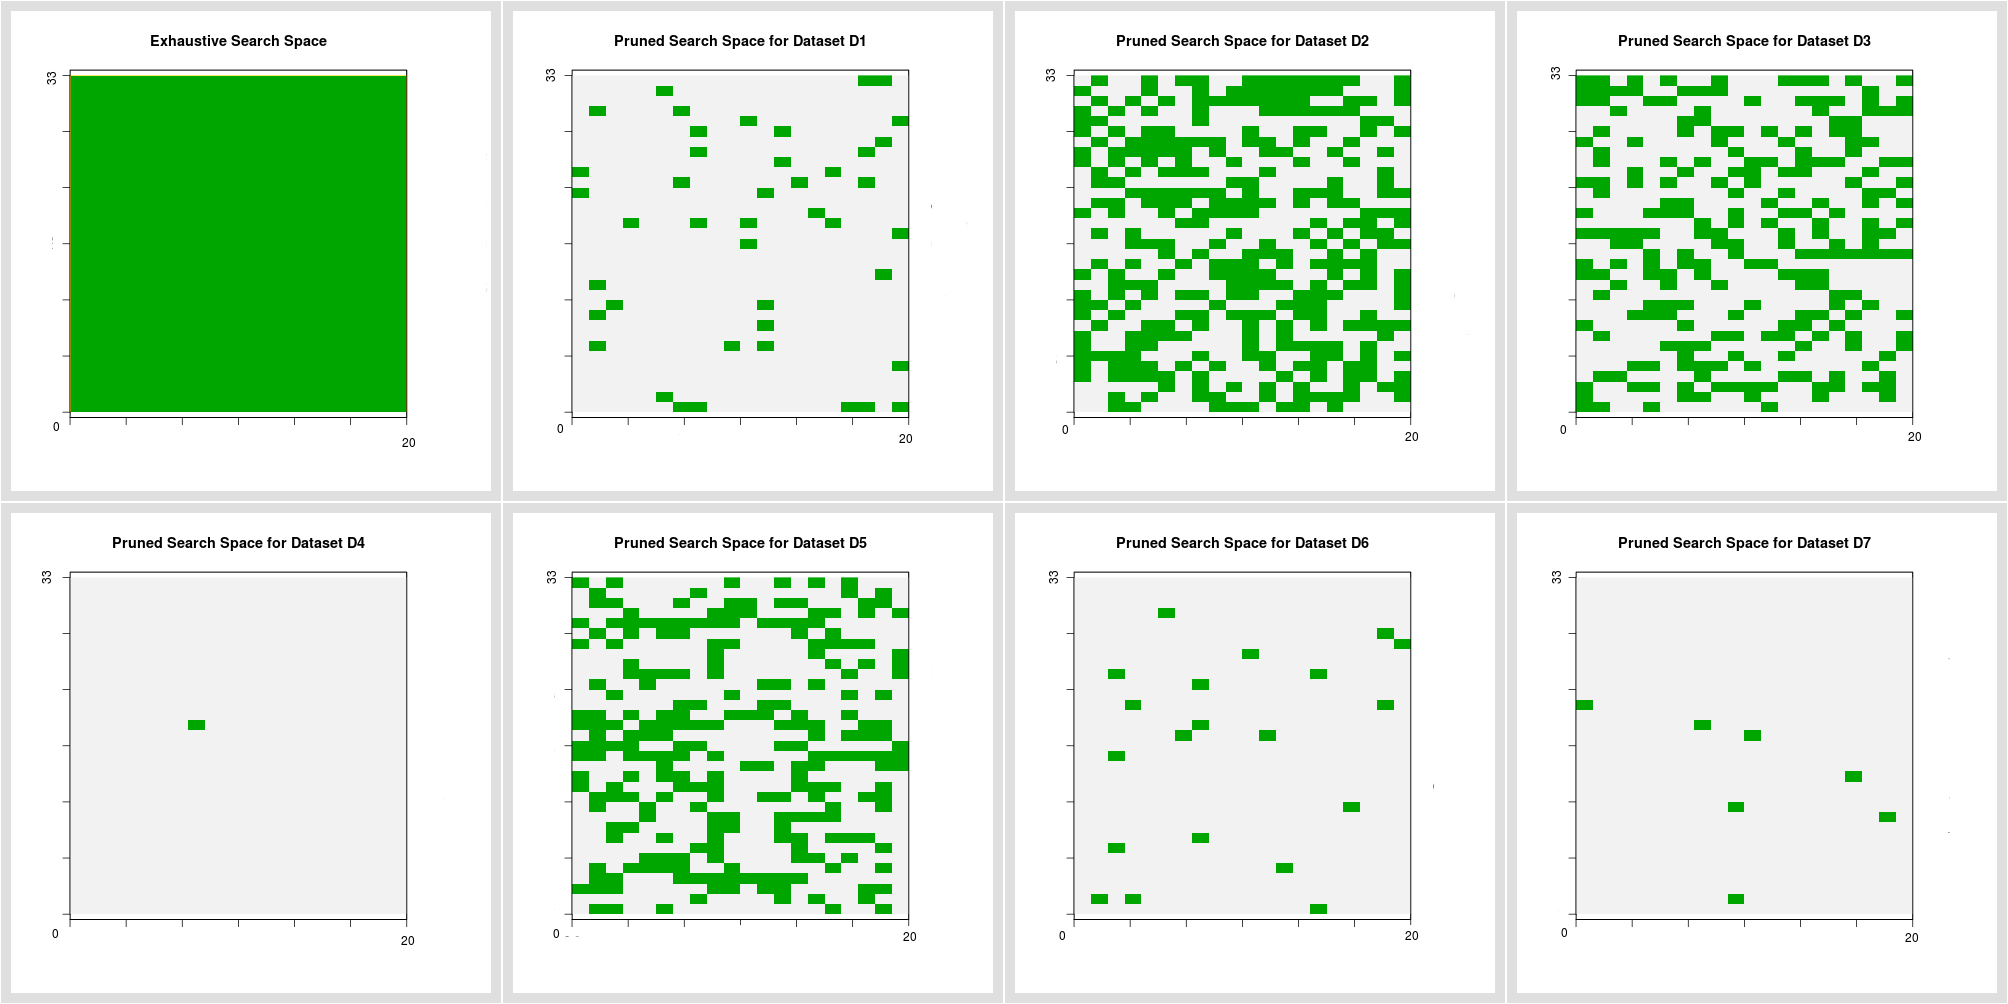
\includegraphics[width=\textwidth]{diversity/montage-clean-pruned-labelled.png}
% \caption{Grid plots showing the exhaustive search space and pruning in search space for different datasets.}
% \label{fig:diversity}
% \end{figure*}

% \subsection{Search Spaces}
% Finally, we compare the various search spaces constructed by discovery algorithm. We represent all people in our experiment universe in a color grid (with 33x20 cells for 660 people). Each cell represents the presence or absence of a person in the search space. If a person was present in the candidate list provided to the tagging algorithm, we color the corresponding cell green, otherwise it is colored white. Figure \ref{fig:diversity} shows the color grids describing search spaces for all datasets, and an exhaustive search space. The positioning of people along the grid is arbitrary, but consistent across grids. Our aim in this visualization is to see the diversity in search spaces created by the algorithm. The purpose of the exhaustive search space is to provide easy comparision to appreciate the reduction in search space. 

% It can be seen that CueNet prunes the search space very differently for different datasets. As we move from dataset to dataset, the data sources present different items of information, and therefore CueNet constructs very search spaces. Dataset D2, D4 and D5 are very large conferences hosting hundreds of people in the same field. This explains why a large portion of the grid is covered. Also, this was the same conference held in three different years, and therefore, had a lot of common attendees resulting in overlap.

% \begin{figure}[t]
% \centering
% 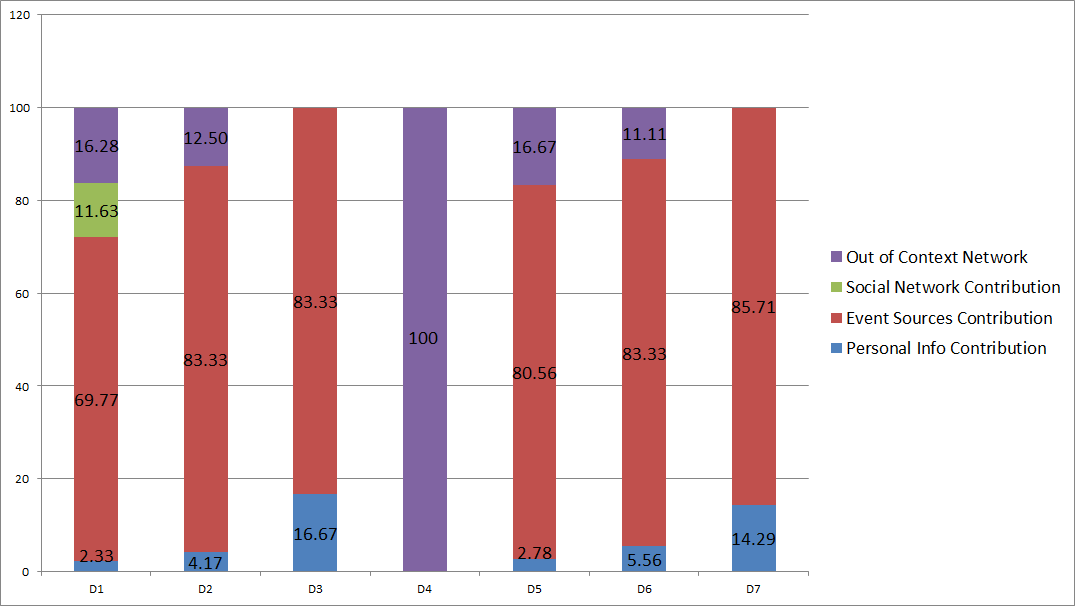
\includegraphics[width=0.9\textwidth]{media/discovery-distro-stacked-2.png}
% \caption{Graph showing the contribution of each source type in context discovery.}
% \label{fig:tag-distribution}
% \end{figure}

% \subsection{Conclusion}
% These experiments validate our three hypotheses. \textbf{First}, Event sources contain a large portion of true positives. From 70\% in D1 to 100\% in D7. There are events for which there is no documentation, and event sources are not able to contribute anything here, as in the case of D4. \textbf{Second}, the discovery algorithm is able to prune the search space using event, personal and social information. The reduction is atleast 50\% for D2 (338 candidates out of 660) but can be very large in some cases (7 candidates for D7). \textbf{Third}, The reduced search space retains a high number of true positives. The hit rate is between 83\% to 100\% (with the exception of D4, where the search space provided no true positives). We also saw how unique the search spaces are, to each dataset, thereby demonstrating the dynamic nature of the algorithm.

\section{Performance Analysis}
In this section, we will look at the performance characteristics of the CueNet algorithm. More specifically, the merge function in the discovery algorithm. In order to achieve this, we will present a generative model to generate large workloads of context networks, which will be merged with each other. Using the generative model, networks of varying sizes will be created so that the time and space complexity of the algorithm can be studied.

\subsection{Generative Models}
\label{section:generative_models}
The generative model requires three main components. A set of places where events occur. An ontology which determines what events occur, and how certain events are more likely to occur as sub-events of already occurring events and the event instances themselves. We will describe each of the components in turn. 


\begin{figure}[t]
\centering
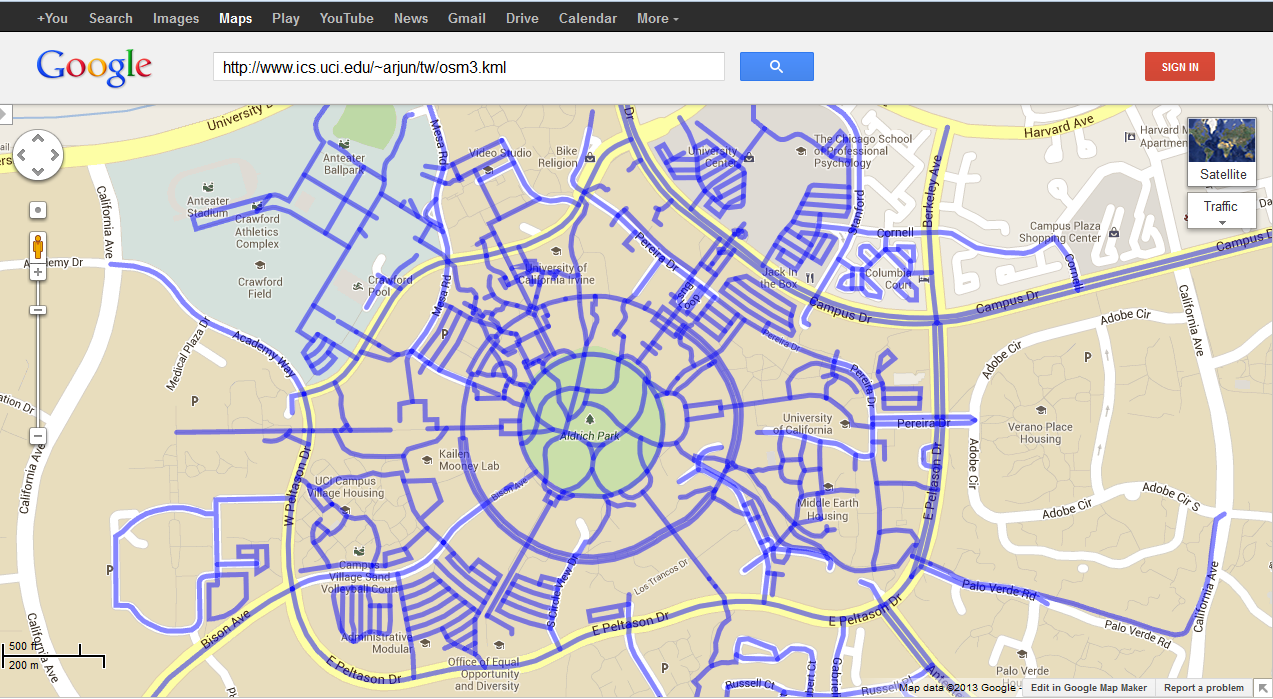
\includegraphics[width=0.9\textwidth]{media/chapter5/perf/map-locations.png}
\caption{Roadmap containing places where events could occur.}
\label{fig:osm-roadmap-uci}
\end{figure}

Instead of designing a generative model for places, it is advisable to use one of these real world databases and select a sample of it to obtain a list of places where events can occur. A large number of place databases are available online. Some commonly used databases are shapefiles \cite{esri:tigerline} for road network information about a particular area. Stanford's SNAP database contains the entire road networks of the USA \cite{stanford:snap}. APIs from websites such as Factual or Yelp.com provide access to large amounts of place information. The FSU dataset available at \cite{fsu:spatial} provides detailed road networks with GPS coordinates from various parts of the country. For our work, we found the spatial database available from OpenStreetMap as the best resource. Their database provides information about road networks, as well as the places themselves. At the same time, data can be downloaded from their website using the download tool or maps for entire cities or states or countries can be downloaded from \cite{cloudmade:download}. The place map of UCI downloaded from their website and converted to KML format is shown in figure \ref{fig:osm-roadmap-uci}. The map data also contains information about different types of objects which can be found on these roads. Please look at their extensive taxonomy \cite{osm:taxonomy} regarding what types of objects can be found here. We select a sample of the nodes in such a network to be our place set.

\begin{figure}[t]
\centering
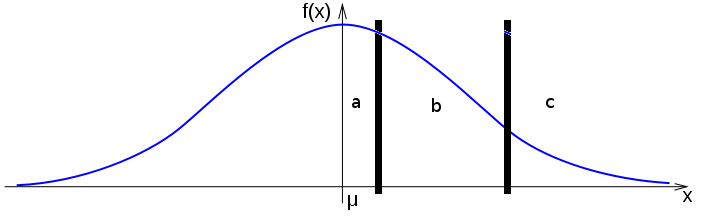
\includegraphics[width=0.9\textwidth]{media/chapter5/perf/gaussian-split.png}
\caption{Gaussian distribution split to generate randon events in ontology.}
\label{fig:gaussian-split}
\end{figure}

The ontology generation module provides three parameters. $O_d$, which controls the depth of subevent trees. $O_{ms}$ which is the maximum number of subevents an event can have. The parameter $D$ is the distribution type. The distribution type decides which events are selected into a hierarchy. A distribution could be Gaussian or Poisson or Uniform distribution. Once the distribution is selected, parameters of the distribution are also provided. We will use a Gaussian distribution as an example to explain the generation of ontologies. But the ideas can be applied to any kind of distribution. 

We want to model events into three categories depending on their general rate of occurrence. Some events are very commonly occurring, a majority of events occur average number of times, and events in the third category occur very rarely. Figure \ref{fig:gaussian-split} shows how a Gaussian random value generator can be used to bucket events into these three zones. The random values are compared with the values $a$, $b$ and $c$. If the $|value|$ is between 0 and $a$, then the event falls into the first category. If it lies between $a$ and $b$, then it lies in the second category. Otherwise it is in the third category.

We consider events in the first category to be atomic events. That is, they occur independently and do not have a subevent hierarchy. An example could be a tweet event or a \texttt{photo-capture} event. We want to create two types of hierarchies. One which is short and fat, and the other which is long and tall. We choose category two to correspond to the former, and category three to contain the latter type of hierarchies. A hierarchy is generated as follows: choose an event, if it is from category 2 or 3, a hierarchy with at most depth $O_d$ and each super event having max $O_{ms}$ subevents is generated. The events are randomly chosen based on their ``real-world'' frequency. These hierarchies are serialized into files. For events in category 3, we double the value of $O_{ms}$. This will allow us to get \textit{fatter} instance hierarchies as we will see later.

In order to generate instances, we randomly select an event based on its ``real-world'' frequency, and load the hierarchy structure from the file, and for subevent class, generate $n$ instances. Thus, if an event $x$ has a subevent $y$ in its hierarchy, then the instance $x_i$ will have subevent instances $\{y_1, y_2 ... y_{|Y|}\}$ where $|Y| < n$. The number $n$ is decided on the basis of an input metric $C$, where for events in category 2, $n = c/2$, and for events in category 3, $n = C$. It must be noted that the $n$ is the maximum number of subevents a super event can contain. The actual number of subevent instances is decided by a uniform random number generator. These hierarchies are serialized into files and stored for the merge tests.

\subsection{Procedure}
In order to understand the time and space complexity of the merge function, we load multiple networks from instance hierarchy into in-memory data structures, and perform a sequence of merges. In order to simulate the workload similar to the discovery algorithm, we select a network, and perform a sequence of merges on it. We will refer to the initially selected network as a \textbf{primary} network and the networks which are merged into it as \textbf{secondary} networks. Thus, given a primary network and a set of secondary networks, we perform the following set of experiments.

First, we fix the size of the primary networks (in terms of node count), and merge secondary networks with varying size, and measure the time taken for the merges to complete.

Second, we fix the size of the primary networks (in terms of depth), and merge secondary networks with varying depth, and measure the time taken for the merges to complete.

Third, we merge a context network with an exact replica of itself, and measure the time taken for the operation. We also change the size of the heap size, and see if there is any effect on the merge operation.

Fourth, we measure the sizes of the networks once they are in memory.

It must be noted that the event instances being used in the experiments do not have event metadata associated with the in-memory instance object. It is assumed that these are being stored separately. The networks used below are simply events with type, spatiotemporal and identification information and references to their subevents and to entities who participate in the events. Any additional information, for example the image object which constitutes the experiential aspect of an event, is stored separately.

We use the following system setup in all our experiments. We use a 8 core Intel(R) Xeon(R) E5504 processor clocking at 2.01Ghz with 8 gigabytes of main memory. We use a single thread to load networks from the file on the disk and proceeds to merge them. The memory footprints of the networks are measured by the classmexer library \cite{classmexer}. The \texttt{Xmx} and \texttt{Xms} JVM parameters were set to be 6000m and 256m respectively.


\begin{figure}[t]
\centering
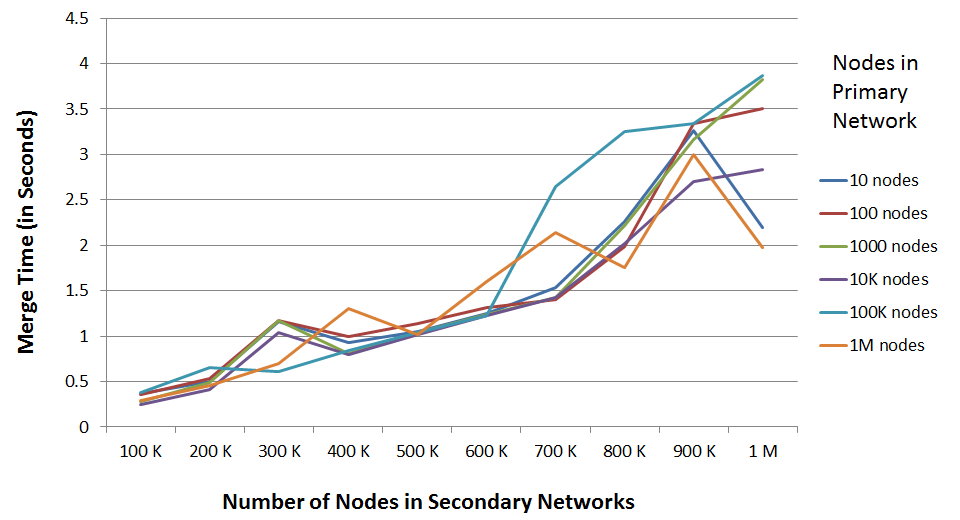
\includegraphics[width=\textwidth]{media/chapter5/axis/perf/mergebignodetest.png}
\caption{Graph showing merge times for different sizes of primary networks.}
\label{fig:agg-merge-tests}
\end{figure}


\subsection{Results}
The graph shown in figure \ref{fig:agg-merge-tests} shows the time taken for merging secondary networks of increasing sizes to a primary network. The size of the primary network is increased from 10 nodes to a million nodes. For each such primary network, a number of secondary networks are merged. As we can see, the size of the primary network does not contribute to the time complexity of the algorithm. This is because the merge algorithm effectively searches the subevent structure to find the node which can best accommodate the secondary network. This is a walk down a single path of the tree. Thus, as long as small secondary networks are obtained from the sources, the merge operations will be less expensive. This is the reason why we tailor our discover queries to provide only very specific information. On the other hand, as the  size of the secondary network increases, we find that the performance increases linearly up to a point, after it which it exponentially increases. This is due to a combination of tree traversal on the secondary network, and the JVM's garbage collector removing outdated objects to accommodate the new objects being created in the primary network. In our implementation, we create new objects in the primary network, as opposed to copying them from the secondary network.

\begin{figure}[t]
\centering
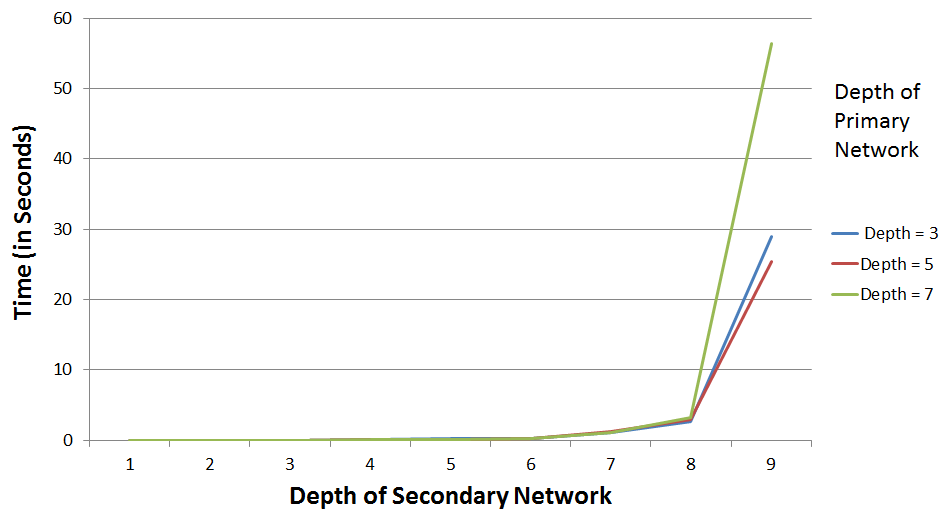
\includegraphics[width=\textwidth]{media/chapter5/axis/perf/mergedepthtest.png}
\caption{Time to merge networks with varying depth.}
\label{fig:agg-depth}
\end{figure}

Similarly, in figure \ref{fig:agg-depth}, we test how merge time varies with increasing depth of the primary network. Here we fix the depth of the primary network to 3, 5 or 7 levels, and load a set of secondary networks from depth 1 to 9. The secondary networks are merged in sequence to the primary network. Each run of the algorithm corresponds to a single primary network (effectively, we reboot the JVM for each primary network). Here the exponential rise after the depth of the secondary network reaches 8 levels is more obvious. This again, shows the importance of constructing selective queries during the \texttt{discover} phase of the algorithm. The loading of all the secondary networks prior to the merge sequence allows us to study the cost of merges in an environment where  memory is not available, and is shared by other citizen objects of the JVM heap. 

Figures \ref{fig:1k-self-merge} and \ref{fig:1m-self-merge} show the time complexity of self merges. A self merge is merging a network with an identical copy of itself. The performance characteristics are very similar to the merge tests seen before.

\begin{figure}[ht]
\begin{minipage}[b]{0.45\linewidth}
\centering
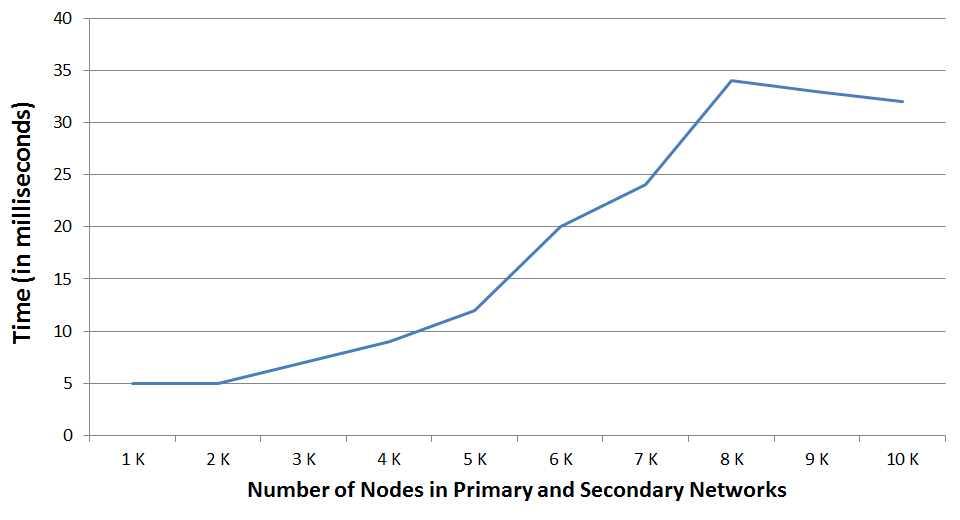
\includegraphics[width=\textwidth]{media/chapter5/axis/perf/selfmerge_10K.png}
\caption{Self Merging Context Networks ($<$ 10K nodes)}
\label{fig:1k-self-merge}
\end{minipage}
\hspace{0.5cm}
\begin{minipage}[b]{0.45\linewidth}
\centering
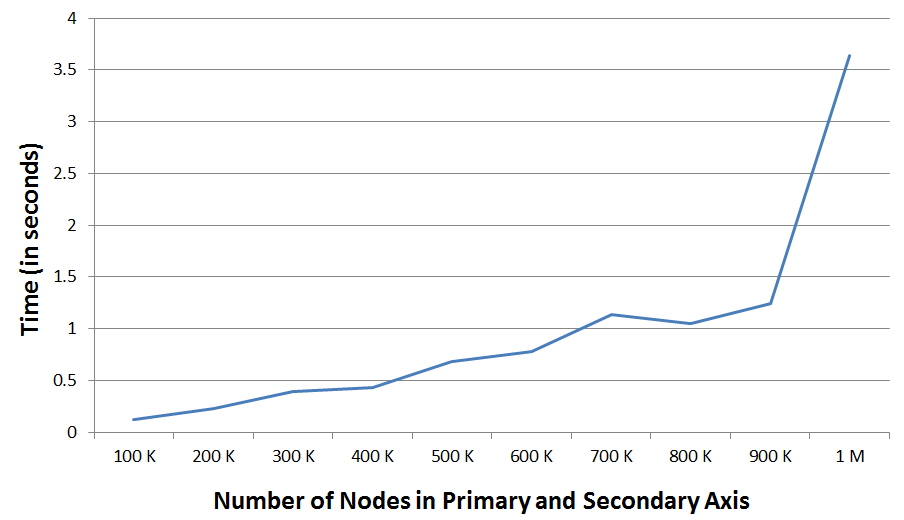
\includegraphics[width=\textwidth]{media/chapter5/axis/perf/selfmerge_1M.png}
\caption{Self Merging Context Networks ($<$ 1M nodes)}
\label{fig:1m-self-merge}
\end{minipage}
\end{figure}

\begin{figure}[t]
\centering
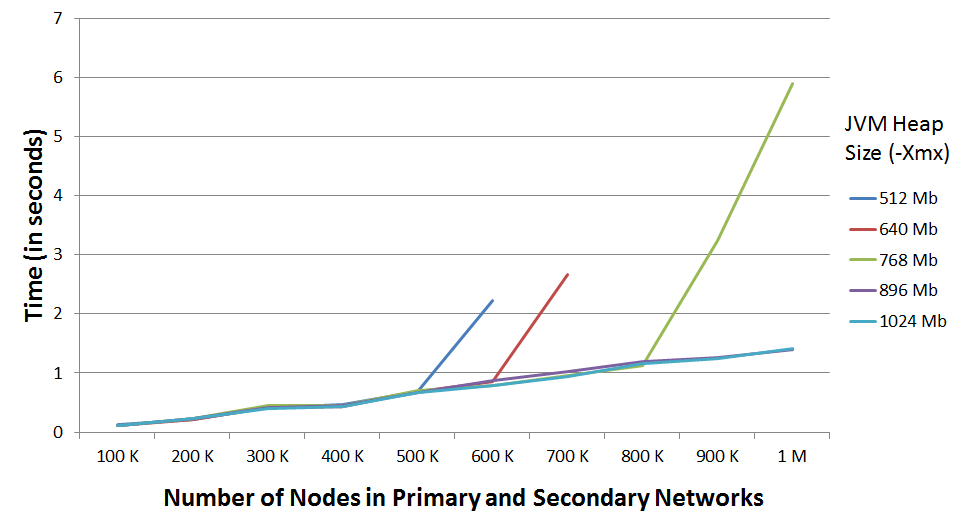
\includegraphics[width=0.9\textwidth]{media/chapter5/axis/perf/selfmerge-increasing-xmx.png}
\caption{Time to merge networks with varying available heap space.}
\label{fig:agg-xmx}
\end{figure}


Now, we will look at how the merges behave with varying heap size (the \texttt{Xmx} runtime parameter provided to the JVM when it is initialized). In figure \ref{fig:agg-xmx}, we see 5 different curves, corresponding to \texttt{Xmx} values of 512m, 640m, 768m, 896m, and 1024m. We load a network twice, perform a merge (a \textit{self-merge}), and record the time the operation takes. The experiment is repeated 5 times for each merge on different randomly created networks. We perform these operations on networks containing 1000, 2000, 3000 nodes up to 700K, 800K, 900K and 1M nodes. As we can see in the figure, we run out of heap space when the networks contain 600K and the Xmx value is 512m. Beyond a 896m, we see that the merge operations only grow linearly, and can be considered a safe limit when self-merges of 1M node networks are to be performed. For heap spaces of less than 896m, the performance time increases exponentially when the network size exceeds 600K nodes. This is, again, because of the creation of nodes in the primary networks.

Finally, we use the Classmexer library \cite{classmexer} to measure the memory footprint of the in-memory context network. We generate random networks of size 1000, 2000 ... 10,000 nodes, and measure the size in kilobytes. The results are shown in figure \ref{fig:sizes}.

\begin{figure}[t]
\centering
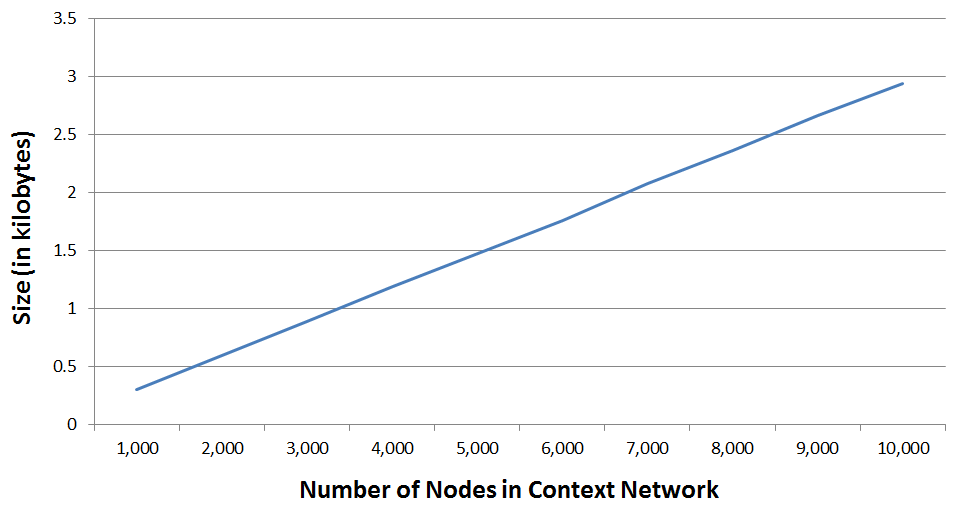
\includegraphics[width=0.9\textwidth]{media/chapter5/axis/perf/size-tree-1000.png}
\caption{Sizes of in-memory context networks contain a few thousand nodes.}
\label{fig:sizes}
\end{figure}


\subsection{Conclusion}

In analyzing the above figures, we have seen that the in-memory merge algorithm performs very well for networks up to 500K nodes. Beyond this point, the performance exponentially decays, both as a combination of large graphs, and the JVM's garbage collector trying to clean up unwanted objects. And therefore it is best recommended to approach an disk based solution or partition the context networks across different machines. 

Since performing many merges (especially with large secondary networks), it is advisable to not perform the merges when the rate of incoming networks is very high. Rather, the system can cache the networks, and extend techniques such as dynamic programming or \textit{batch merges} to improve the overall performance. Such an algorithm, does not already exist, and can prove to be a very important future research problem to improve the utility of context networks in various domains with large workloads.

% \begin{figure}[ht]
% \begin{minipage}[b]{0.45\linewidth}
% \centering
% 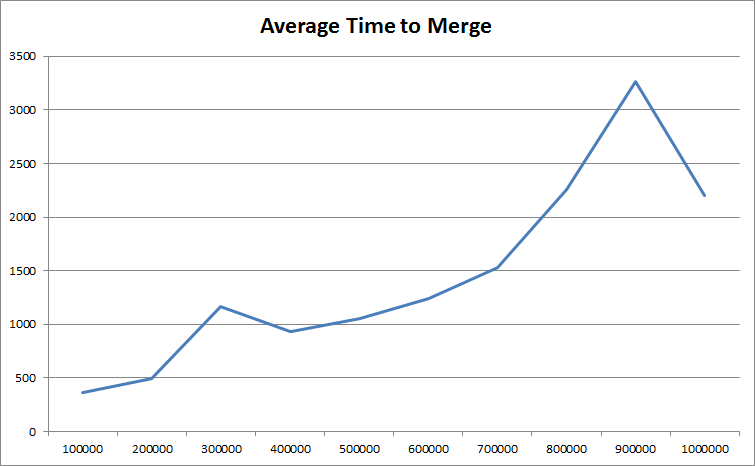
\includegraphics[width=\textwidth]{media/chapter5/perf/mergebignodetest_10.png}
% \caption{10 Nodes}
% \label{fig:pic1}
% \end{minipage}
% \hspace{0.5cm}
% \begin{minipage}[b]{0.45\linewidth}
% \centering
% 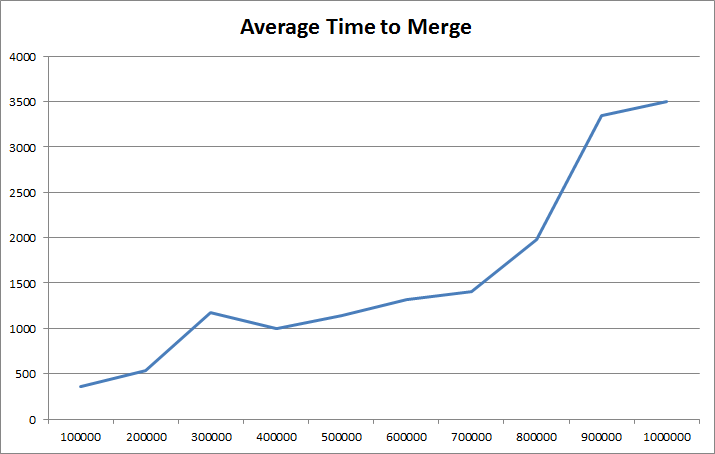
\includegraphics[width=\textwidth]{media/chapter5/perf/mergebignodetest_100.png}
% \caption{100 Nodes}
% \label{fig:pic2}
% \end{minipage}

% \begin{minipage}[b]{0.45\linewidth}
% \centering
% 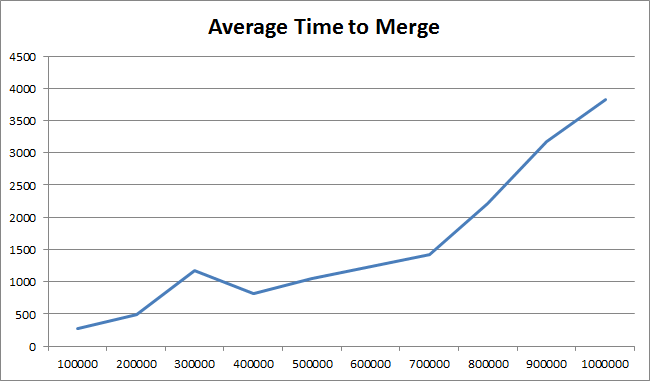
\includegraphics[width=\textwidth]{media/chapter5/perf/mergebignodetest_1000.png}
% \caption{10 Nodes}
% \label{fig:pic1}
% \end{minipage}
% \hspace{0.5cm}
% \begin{minipage}[b]{0.45\linewidth}
% \centering
% 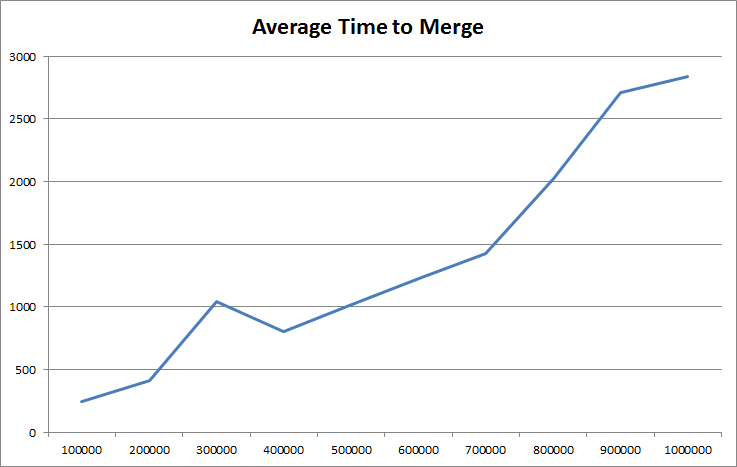
\includegraphics[width=\textwidth]{media/chapter5/perf/mergebignodetest_10K.png}
% \caption{100 Nodes}
% \label{fig:pic2}
% \end{minipage}

% \begin{minipage}[b]{0.45\linewidth}
% \centering
% 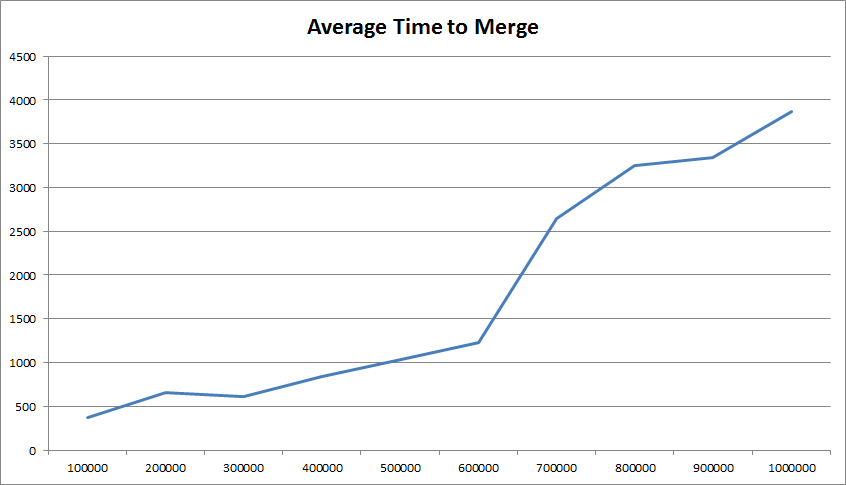
\includegraphics[width=\textwidth]{media/chapter5/perf/mergebignodetest_100K.png}
% \caption{100K Nodes}
% \label{fig:pic2}
% \end{minipage}
% \hspace{0.5cm}
% \begin{minipage}[b]{0.45\linewidth}
% \centering
% 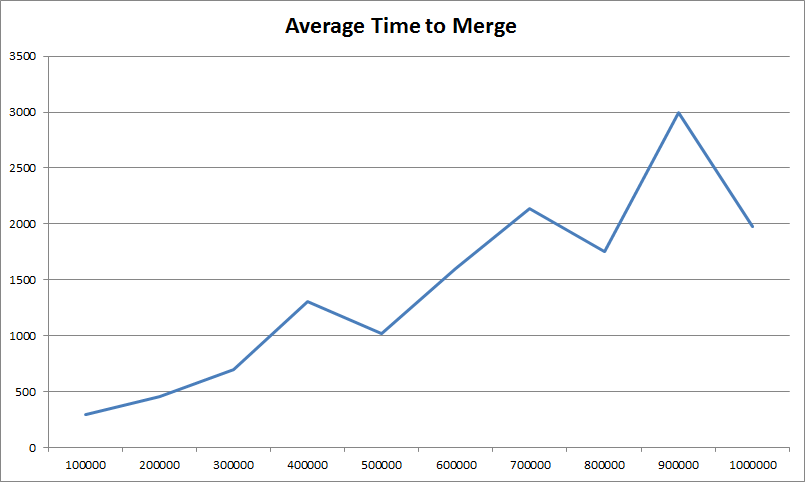
\includegraphics[width=\textwidth]{media/chapter5/perf/mergebignodetest_1M.png}
% \caption{1M Nodes}
% \label{fig:pic3}
% \end{minipage}
% \end{figure}


% \begin{figure}[ht]
% \begin{minipage}[b]{0.28\linewidth}
% \centering
% 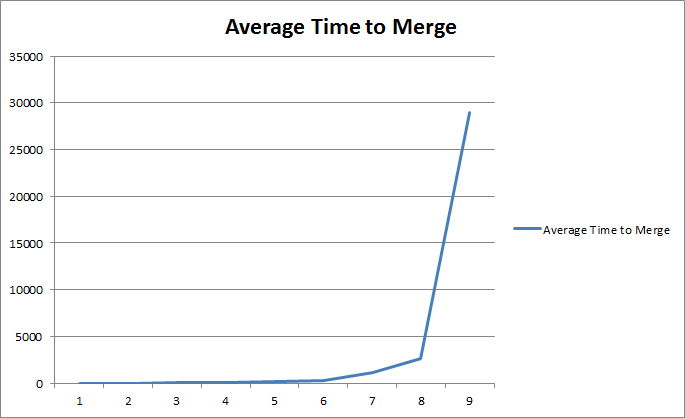
\includegraphics[width=\textwidth]{media/chapter5/perf/mergedepthtest_3.png}
% \caption{depth = 3}
% \label{fig:pic1}
% \end{minipage}
% \hspace{0.5cm}
% \begin{minipage}[b]{0.28\linewidth}
% \centering
% 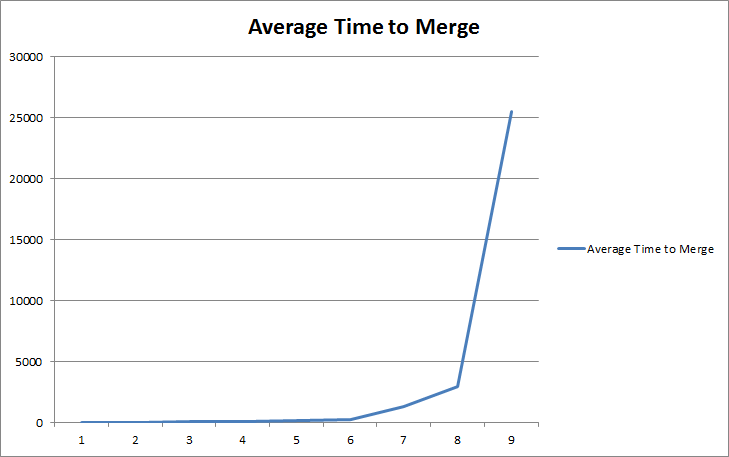
\includegraphics[width=\textwidth]{media/chapter5/perf/mergedepthtest_5.png}
% \caption{depth = 5}
% \label{fig:pic2}
% \end{minipage}
% \hspace{0.5cm}
% \begin{minipage}[b]{0.32\linewidth}
% \centering
% 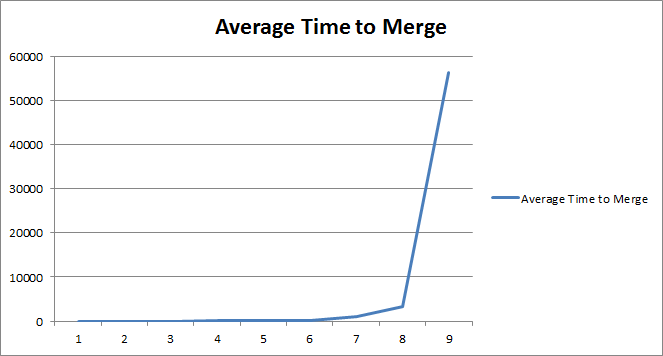
\includegraphics[width=\textwidth]{media/chapter5/perf/mergedepthtest_7.png}
% \caption{depth = 7}
% \label{fig:pic3}
% \end{minipage}

% \end{figure}